\section{Pedagogical Design}
\label{sec:pedagogy}

Each design choice described in Sections~\ref{sec:architecture}
and~\ref{sec:quantum-simulator} was made with a specific misconception or missing intuition in
mind, in the spirit of Papert's constructionism~\cite{papert1980mindstorms}: a learner
constructs a working artifact and inspects its behavior directly, rather than observing that
behavior secondhand.

\textbf{Placing gates as physical blocks, not dragging icons onto a schematic.} A gate
occupies a specific block placed a specific number of steps east of a qubit line's anchor, and
right-clicking it cycles through its available presets in a fixed order. This arrangement is
closer to physically assembling an apparatus than to editing a diagram on a screen: a player
who wants to compare a Hadamard gate against a Pauli-$X$ gate must actually remove one block
and place (or cycle to) the other, in the same spirit that CircuitCraft asks a player to wire
and re-wire physical blocks rather than click a schematic's component library.

\textbf{An explicit distinction between an ideal readout and a real measurement.} A common
early misconception is treating ``the quantum state'' and ``what you measure'' as the same
thing, when the entire pedagogical point of measurement collapse is that they are not.
QuantumCraft's probe deliberately exposes both as separate, differently-labeled interactions
-- a plain right-click for the full, exact probability distribution (something no physical
quantum computer could ever hand a user directly), and a shift-right-click for a single,
collapsing, irreversible sample from that distribution -- so that a player must deliberately
choose which question to ask, rather than the mod quietly picking one on their behalf.
Figure~\ref{fig:hud} shows the resulting heads-up display for a Bell-state circuit
(Section~\ref{sec:exp-bell}) in each mode.

\begin{figure}[htbp]
\centering
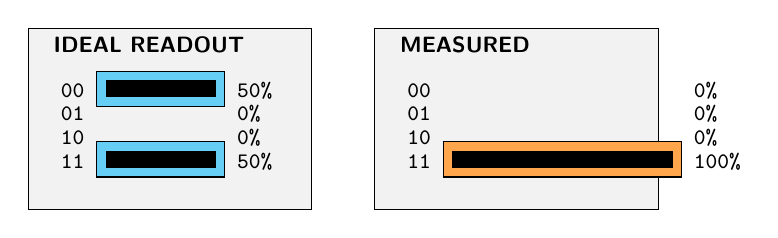
\begin{tikzpicture}[font=\footnotesize\ttfamily]
\begin{scope}
\node[draw, fill=gray!10, minimum width=3.6cm, minimum height=2.3cm, align=left, anchor=north west, inner sep=4pt] (idealbox) at (0,0) {};
\node[anchor=north west, font=\footnotesize\sffamily\bfseries] at (idealbox.north west) {\ \ IDEAL READOUT};
\node[anchor=north west] at ([yshift=-0.42cm]idealbox.north west) {\ \ 00\ \fcolorbox{black}{cyan!60}{\rule{1.4cm}{2.2mm}}\ 50\%};
\node[anchor=north west] at ([yshift=-0.72cm]idealbox.north west) {\ \ 01\ \phantom{\fcolorbox{black}{cyan!60}{\rule{1.4cm}{2.2mm}}}\ 0\%};
\node[anchor=north west] at ([yshift=-1.02cm]idealbox.north west) {\ \ 10\ \phantom{\fcolorbox{black}{cyan!60}{\rule{1.4cm}{2.2mm}}}\ 0\%};
\node[anchor=north west] at ([yshift=-1.32cm]idealbox.north west) {\ \ 11\ \fcolorbox{black}{cyan!60}{\rule{1.4cm}{2.2mm}}\ 50\%};
\end{scope}
\begin{scope}[xshift=4.4cm]
\node[draw, fill=gray!10, minimum width=3.6cm, minimum height=2.3cm, align=left, anchor=north west, inner sep=4pt] (measbox) at (0,0) {};
\node[anchor=north west, font=\footnotesize\sffamily\bfseries] at (measbox.north west) {\ \ MEASURED};
\node[anchor=north west] at ([yshift=-0.42cm]measbox.north west) {\ \ 00\ \phantom{\fcolorbox{black}{orange!70}{\rule{2.8cm}{2.2mm}}}\ 0\%};
\node[anchor=north west] at ([yshift=-0.72cm]measbox.north west) {\ \ 01\ \phantom{\fcolorbox{black}{orange!70}{\rule{2.8cm}{2.2mm}}}\ 0\%};
\node[anchor=north west] at ([yshift=-1.02cm]measbox.north west) {\ \ 10\ \phantom{\fcolorbox{black}{orange!70}{\rule{2.8cm}{2.2mm}}}\ 0\%};
\node[anchor=north west] at ([yshift=-1.32cm]measbox.north west) {\ \ 11\ \fcolorbox{black}{orange!70}{\rule{2.8cm}{2.2mm}}\ 100\%};
\end{scope}
\end{tikzpicture}
\caption{Schematic reconstruction of the probe's result heads-up display for the Bell-state
circuit of Section~\ref{sec:exp-bell}. Left: a plain right-click's ideal readout, showing the
exact 50/50 split between $|00\rangle$ and $|11\rangle$ with zero probability at
$|01\rangle$/$|10\rangle$. Right: a shift-right-click's measurement, collapsing to a single
sampled outcome (here $|11\rangle$) highlighted in a distinct color, with every other row at
0\%.}
\label{fig:hud}
\end{figure}

\textbf{A gate set small enough to reason about by hand, large enough to entangle and
interfere.} Six single-qubit presets and a two-marker multi-qubit mechanism are enough to
build every worked experiment in Section~\ref{sec:experiments} -- a superposition, an
entangled Bell pair, a phase-kickback interference effect, a three-qubit GHZ state, and a
Toffoli-gate truth table -- while remaining small enough that a student can, in principle,
multiply out every $2\times2$ or $4\times4$ matrix involved by hand and check the mod's
answer, the same verification discipline Section~\ref{sec:validation} itself uses. A larger
gate set (arbitrary rotation angles, for instance) was deliberately deferred
(Section~\ref{sec:limitations}) in favor of a fixed palette that keeps this hand-verifiability
intact.

\textbf{A hard cap of three qubits.} Restricting the register to at most three qubits keeps
every worked circuit's full $2^n$-dimensional statevector small enough to display every basis
state's probability at once in the result heads-up display (Figure~\ref{fig:hud}), rather than
requiring the player to scroll or select a subset of a much larger state space, while still
being large enough to demonstrate every multi-qubit phenomenon in this mod's scope: two
qubits are the minimum needed for entanglement at all, and three are the minimum needed for
both the Toffoli gate and a GHZ state.
